\documentclass[11pt,a4paper]{article}

\usepackage{amsmath}
\usepackage{amsfonts}
\usepackage{amssymb}
\usepackage{graphicx}
\usepackage[left=30mm,right=30mm,top=35mm,bottom=35mm]{geometry}
\linespread{1.05}
\graphicspath{{images/}}


\begin{document}

\newcommand{\N}{\mathbb{N}}
\newcommand{\R}{\mathbb{R}}
\newcommand{\Z}{\mathbb{Z}}
\newcommand{\e}{\varepsilon}
\newcommand{\bb}[1]{\boldsymbol{#1}}

\section{HB and HB+}

HB is an authentication protocols first introduced by Blum et al. \cite{10.1007/3-540-45682-1_4}, \cite{10.1007/3-540-48329-2_24} that relies on the hardness of the learning parity with noise problem (LPN) for security and is provably secure against passive attacks. 

A modification of the HB protocol in order for it to be secure against an active adversary is the HB+ protocol by Juels and Weis \cite{juels2005authenticating}.

\subsection{Protocols}

Figure \ref{fig1} shows one iteration of the authentication of HB.

\begin{figure}[h]
	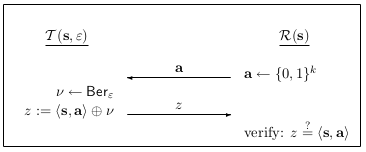
\includegraphics[width=8cm]{hb}
	\centering
	\caption{One iteration of the HB protocol}
	\label{fig1}
\end{figure}

A tag $\mathcal{T}$ and a reader $\mathcal{R}$ share a random secret key $\bb{s} \in \{0,1\}^k$. One of the $n$ iteration (all of which happen in parallel) of the authentication step consists of the following:
$\mathcal{R}$ sends a random challenge $\bb{a} \in \{0,1\}^k$ to $\mathcal{T}$ who in turn calculates $\bb{z}:= \langle \bb{s}, \bb{a} \rangle \oplus v$ with $v \leftarrow \mathsf{Ber}_\e$.
This result is sent back to $\mathcal{R}$ who then calculates if the iteration is \textit{successful}, i.e. $\bb{z} = \langle \bb{s}, \bb{a} \rangle $. 
Notice that even iterations of an honest tag using the correct key $s$ can be unsuccessful with probability $\e$. The reader therefore accepts the authentication of the tag if the number of unsuccessful iterations is at most $\approx \e \cdot n$. \\\\
Figure \ref{fig2} shows one iteration of the authentication of HB+.

\begin{figure}[h]
	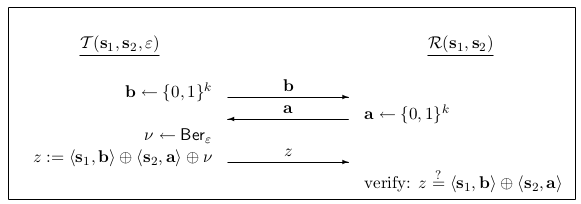
\includegraphics[width=11cm]{hbp}
	\centering
	\caption{One iteration of the HB+ protocol}
	\label{fig2}
\end{figure}

 $\mathcal{R}$ and $\mathcal{T}$ now share two secret keys $\bb{s_1}, \bb{s_2} \in \{0,1\}^k$. One iteration of the authentication step now looks as follows:
$\mathcal{T}$ first sends a random "blinding factor" $\bb{b} \in \{0,1\}^k$ to $\mathcal{R}$. The reader then, as for HB, sends a random challenge $\bb{a} \in \{0,1\}^k$ to $\mathcal{T}$ who in turn calculates $z:= \langle \bb{s_1}, \bb{b} \rangle \oplus \langle \bb{s_2}, \bb{a} \rangle \oplus v$ with $v \leftarrow \mathsf{Ber}_\e$.
This result is sent back to $\mathcal{R}$ who then calculates if the iteration is \textit{successful}, i.e. $z = \langle \bb{s_1}, \bb{b} \rangle \oplus \langle \bb{s_2}, \bb{a} \rangle$. 
Again, even if $\mathcal{T}$ sends an honest $z$ using the correct keys $\bb{s_1}$, $s_2$ the iteration can be \textit{unsuccessful}. Therefore, up to $\approx e \cdot n$ \textit{unsuccessful} iterations are allowed fot the tag to still be accepted.

\subsection{Implementation}

We implemented different versions of HB and HB+ in order to investigate different degrees of parallelism and their effect on the performance on the Arduino Uno. For the parameters we worked with the suggested values given in \cite{armknecht} and looked at 80-bit and 128-bit security.

First, we implemented the naive version where the Tag receives one challenge at a time to use with the first two sets of parameters (for HB and HB+ respectively). 
Then we implemented the improved version suggested in \cite{hbsharp} that required a slight modification to precompute $r$ noise bits where the number of 1s is less than $u \cdot r$ to use the third set of parameters reducing the number of rounds to 256 \cite{hbsharp}.

Our parallel implementation of HB and HB+ introduces a parameter \textit{maxChallenge} to set the number of challenges sent at a time. 
Notice that sending all challenges at once would be infeasible since we would have to send $k \cdot r$ which, in the case of $ k = 512$ and $r = 441$ bits, would be $512 \cdot 441 = 225.792$ bits or $27$ kB while the Arduino Uno only has 2 kB of SRAM. 
The highest number for maxChallenges would be 32 but since other variables of the program also occupy space, the realistic number can be found at around 22 for HB and 18 for HB+ assuming 80-bit security. 
 

\section{AUTH}

The AUTH protocol shown in Figure \ref{fig3} was introduced by Kiltz et al. \cite{Kiltz2017} and represents a two-round authentication protocol secure against active attacks and man-in-the-middle attacks, even in a quantum setting. The security of this protocol relies on the hardness of the \textit{subspace LPN problem} which is reducible to the generic LPN problem.

\subsection{Protocols}

\begin{figure}[h]
	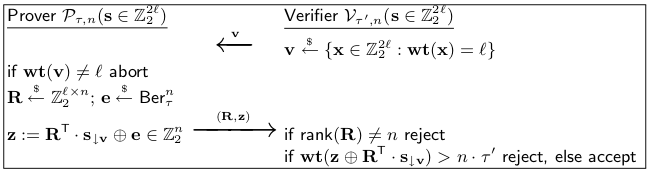
\includegraphics[width=12cm]{auth}
	\centering
	\caption{Two-round authentication protocol AUTH}
	\label{fig3}
\end{figure}

Whereas the random challenges $\bb{R} \in \Z_2^{l \times n}$ (each row of the matrix $\bb{R}^T$ corresponding to one challenge $a$ in HB) were computed by the Verifier $\mathcal{V}$ in HB, they are now computed by the Prover $\mathcal{P}$.
$\mathcal{V}$ instead sends a random vector $\bb{v} \in \Z_2^{2l}$ with Hamming weight $\text{wt}(\bb{v}) = l$ to select $l$ of the $2l$ key bits of $s$ to produce a key subset $\bb{s}_{\downarrow v}$ which is derived from $\bb{s}$ by deleting all bits $\bb{s}[i]$ where $\bb{v}[i] = 0$.
Then, $\bb{z} \in \Z_2^n$ is computed as $\bb{R}^T \cdot \bb{s}_{\downarrow v} \oplus \bb{e}$ and sent to $\mathcal{V}$ along with $\bb{R}$.
$\mathcal{V}$ rejects the authentication if either $\text{rank}(\bb{R}) \neq n$ or if the number of unsuccessful iterations denoted as $\text{wt}(\bb{z} \oplus \bb{R}^T \cdot \bb{s}_{\downarrow v})$ is greater than the threshold $n \cdot \tau'$ with $\tau' = 0.25 + \tau/2$.

\subsection{Implementation}

We implemented two versions of AUTH: the standard version given in Figure \ref{fig3} and a variation that uses blinding vectors to avoid checking rank as given in \cite{Kiltz2017}. 
Using a typical set of parameters $l=500$, $n=250$, $\lambda = 80$ we quickly realized that sampling a challenge matrix in $\Z_2^{l \times n}$ would be infeasible since one would need to store $500 \cdot 250$ = 125.000 bits or 15 kB while the Arduino only has 2kB of SRAM. We therefore deemed the protocol infeasible for our purpose of implementing it on the limited Arduino Uno together with MAC1 and MAC2 which use the same structure.


\section{Lapin}

\subsection{Protocol}

The protocol is defined over the ring $R = F_2[X] / (f)$. Both the honest tag $\mathcal{T}$ and the reader $\mathcal{TR}$ hold $s, s' \in R$ as the secret key, $\tau$ and $\tau'$ denote the bias for the Bernoulli distribution $\mathsf{Ber}_\tau$ and the acceptance threshold. The two-round procedure is shown in \ref{fig4}.

\begin{figure}[h]
	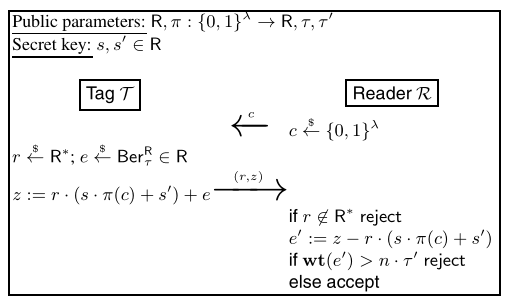
\includegraphics[width=9.5cm]{lapin}
	\centering
	\caption{Two-round authentication protocol Lapin}
	\label{fig4}
\end{figure}

$\mathcal{R}$ first sends a bitstring $c$ of length $\lambda$ to $\mathcal{T}$. $\mathcal{T}$ then samples an element $r$ uniformly from the ring $R$ and an element $e$ that has its coefficients drawn independently from $\mathsf{Ber}_\tau$. 
$\mathcal{T}$ then calculates $z$ as in Figure \ref{fig4} where a mapping function $\pi: \{0,1\}^\lambda \rightarrow R$ maps c to an element of the ring. 
$\mathcal{R}$ finally receives $r$ and $z$ from $\mathcal{T}$ and counts the number of bits that are different between $z$ and its own calculation of $z$ without the noise. 
If the number is greater than $n \cdot \tau$ ($n$ denotes the degree of f) then the authentication is rejected, otherwise it is accepted.


\subsection{Implementation}

The original paper \cite{lapin} gives two possible implementations, one that uses a reducible polynomial for $f$ and one that uses an irreducible one.
We chose the former version because it is more efficient. Even though it requires a higher code size as a trade-off for faster response time, flash memory is not a scarce resource on the Arduino Uno with regards to this lightweight protocol. 

Given that $f$ factors into distinct irreducible factors $f_1,\dots ,f_m$, we can perform more efficient multiplications in the ring using the CRT (Chinese Remainder Theorem) representation $\hat{a} = (a \mod f_1, \dots ,f_m)$ of the elements in $F_2[X] / (f)$ which is why this version has an edge over the one using an irreducible $f$ regarding performance. 
The paper suggests using a reducible polynomial $f$ to define the ring $R = F_2[X] / (f)$ that is the product of $m = 5$ irreducible pentanomials where the numbers specify the coefficients that are non-zero: (127,8,7,3,0), (126,9,6,5,0), (125,9,7,4,0), (122,7,4,3,0), (121,8,5,1,0). 
The mapping $\pi: \{0, 1\}^{80} \rightarrow R$ is defined as $\pi(c) = (v_1,\dots, v_5)$ where we get $v_i \in F_2[X] / (f_i)$, $1 \leq i \leq 5$ by  padding $c \in \{0,1\}^{80}$ with $deg(f_i) - 80$ zeros.
Similar to the implementation laid out in the original paper, we used the right-to-left comb multiplication from \cite{hankerson}. We also wrote a normal multiplication function and another sparse multiplication function for multiplication with $\pi(c)$ which is twice as fast as the former by abusing the fact that only the first 80 bits can be non-zero.




\newpage
\addcontentsline{toc}{section}{\refname}
\bibliographystyle{alpha}
\bibliography{references}

\end{document}
